\documentclass[etd,oneside,senior]{BYUPhys}
\usepackage{pdfpages}
\usepackage{listings}
\usepackage[outputdir=out]{minted}
\usepackage{fontspec}
\graphicspath{{./figures}}
\DeclareMathOperator{\J}{J}
\DeclareMathOperator{\struveh}{H}

% Hypergeometric function command (from https://tex.stackexchange.com/a/2477)
\newcommand*\pFqskip{8mu}
\catcode`,\active
\newcommand*\pFq{\begingroup
        \catcode`\,\active
        \def ,{\mskip\pFqskip\relax}%
        \dopFq
}
\catcode`\,12
\def\dopFq#1#2#3#4#5{%
        {}_{#1}F_{#2}\biggl[\genfrac..{0pt}{}{#3}{#4};#5\biggr]%
        \endgroup
}

% If you'd like to print your thesis using double-sided printing,
% remove the etd option and change the oneside argument to twoside, like this:
%
%\documentclass[twoside,masters]{BYUPhys}

% Your name
  \Author{Michael Greenburg}

% Enter the year your thesis is approved (for senior thesis or capstone)
  \Year{2024}

% If you have a long title, split it between multiple lines using the \\ command
  \Title{Title: Titles Must Be in Mixed Case and May Not Exceed Six Inches on One Line\\
  and Must Be in the Inverted Pyramid Format When\\
  Additional Lines Are Needed
  }

% Your research advisor
\AdvisorTitle{Advisors}
  \Advisor{Steven Turley, David Allred}

% The text of your abstract
  \Abstract{The abstract is a summary of the thesis/dissertation
  with emphasis on the findings of the study. The abstract must not
  exceed 350 words in length and fit on one page, single spaced.
  
  Comptational optics things. Didn't work, to make it work I think the impedance matrix condition number needs to be reduced somehow}

 \Keywords{mirror, reflect}

% Acknowledge those who helped and supported you
  \Acknowledgments{
    Acknowledgements should be simple, in good taste, and fit on one page
  }

%% The members of your committee (masters only need A and B, PhD need all 4)
%  \MemberA{Committee Member A}
%  \MemberB{Committee Member B}
%  \MemberC{Committee Member C}
%  \MemberD{Committee Member D}
%

\begin{document}

% Start page counting in roman numerals
\frontmatter

% This command makes the formal preliminary pages.
% You can comment it out during the drafting process if you want to save paper.
\makepreliminarypages

% Make the table of contents.
\tableofcontents

% Start regular page counting at page 1
\mainmatter





% INTRO %%%%%%%%%%%%%%%%%%%%%%%%%%%%%%%%%%%%%%%%%%%%%%%%%%%%%%%%%%%%%%%%%%%%%%%%%%%%%%%%%%%%%%%%%%%%%%%%%%%%%%%%%%%%%%%%

\chapter{Introduction} \label{chap:intro}

\section{The Problem} \label{sec:problem}

We don't have good models of how roughness affects reflectance (CITE). There's stuff that does well when the roughness is a lot bigger or smaller than the wavelength of incident light (CITE both, expand on this); this is meant to fit between.



\section{The Attempted Solution} \label{sec:attempted_solution}

Made a computational model for circular rough mirrors. It's available on \href{https://github.com/mjg0/Mirrors.jl}{GitHub}.

%%%%%%%%%%%%%%%%%%%%%%%%%%%%%%%%%%%%%%%%%%%%%%%%%%%%%%%%%%%%%%%%%%%%%%%%%%%%%%%%%%%%%%%%%%%%%%%%%%%%%%%%%%%%%%%%%%%%%%%%





% EXPECTED RESULTS %%%%%%%%%%%%%%%%%%%%%%%%%%%%%%%%%%%%%%%%%%%%%%%%%%%%%%%%%%%%%%%%%%%%%%%%%%%%%%%%%%%%%%%%%%%%%%%%%%%%%

\chapter{Methods} \label{chap:math}

\section{Modeling Expected Results} \label{sec:expected_results}

We need to make sure that our results make sense--does our program predict correct reflectance even for a flat mirror? So we need to figure out an equation that gives us what we expect: given an incident beam angle, $\alpha$, how would an ideal mirror react to uniform illumination? In the far field, what is the intensity (as predicted by physical optics) at a certain polar and azimuthal angle?

\subsection{Huygens Approximation} \label{subsec:huygens_approx}

We obviously need an expected reflectance profile to make sure that what we're doing looks right. Since a flat, finite, perfectly conductive mirror is just the reflective version of an aperture (CITE), we can use the Huygens-Fresnel principle to see how light should behave when it hits a perfectly flat, perfectly reflective mirror.

Unfortunately I couldn't find an equation for diffraction through a \textit{tilted} circular aperture so I had to figure it out myself. An easy test of what I found is ensuring that whatever I come up with is identical to the circular aperture diffraction when the light comes in normal to the mirror, which is proportional to (CITE):

\begin{equation}\label{eq:airy}
  \frac{\J_1(kR\sin(\theta))}{kR\sin(\theta)}
\end{equation}

\ldots where $k$ is the wave number, $\frac{2\pi}{\lambda}$ ($\lambda$ being the wavelength), $R$ is the radius of the aperture (mirror in our case), and $\theta$ is the angle at which the reflectance is measured. $J_1$ is the first order Bessel function of the first kind. This is the Airy pattern (CITE?).

\subsection{Setup} \label{sec:setup}

The electric field on a flat mirror in the x-y plane due to a plane wave coming in at an angle $\alpha$ from normal (the z axis), inclined toward the x axis, is proportional to (CITE?):

\begin{equation}
  e^{ikx\sin\left({\alpha}\right)}
\end{equation}

The contribution of one point on the mirror to the far field reflectance at some polar angle $\theta$ and azimuthal angle $\phi$ is just going to be that exponential multiplied by some phase shift.

\subsection{Phase Shift} \label{sec:phase_shift}
Since we're concerned with reflectance in the far field, all we need to determine is the phase shift relative to the origin. For some point $p$, we need to calculate the distance $d$ between that point and the origin \textit{along the direction of travel toward the point in the far field} defined by $\theta$ and $\phi$.

\begin{figure}
  \centerline{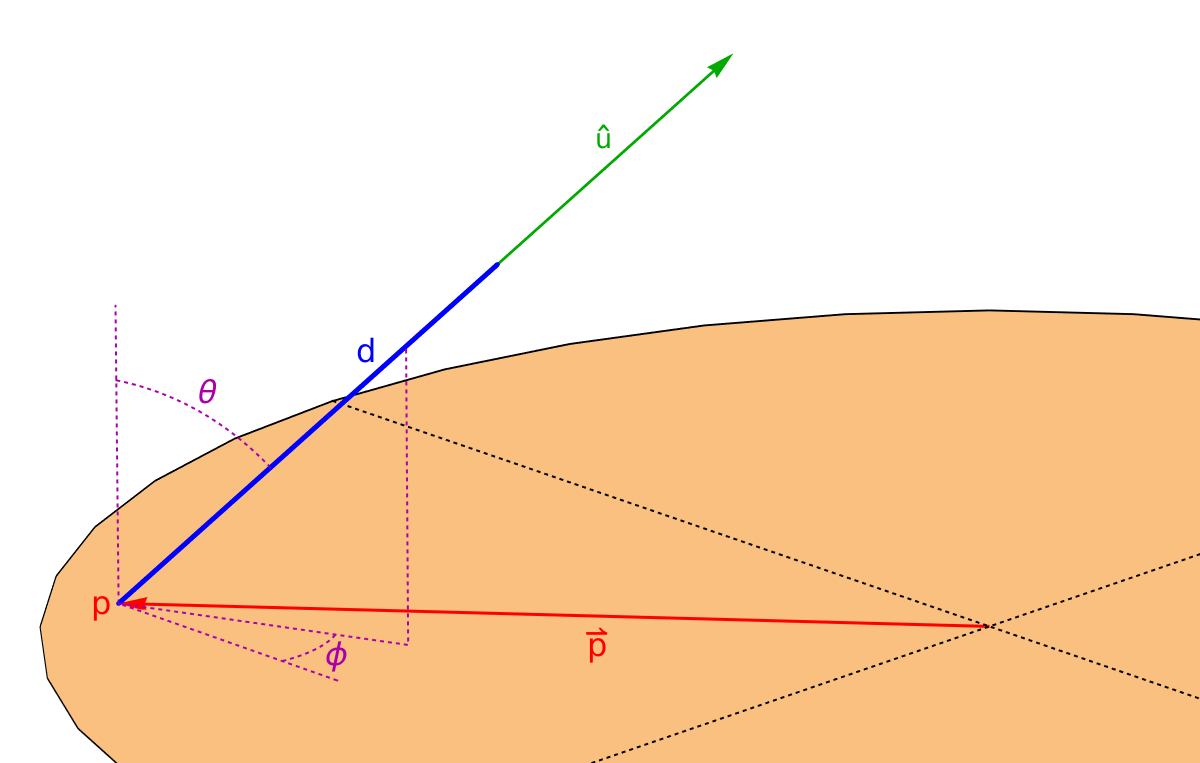
\includegraphics[width=\textwidth]{phase-length}}
  \caption[Phase length of a beam of light]{\label{fig:phase_length}
    $d$ is the phase shift of light coming from $p$ relative to light coming from the origin.}
\end{figure}

$d$ is given by dotting the unit vector $\hat{u}$ with $-\vec{p}$ [\ref{fig:phase_length}]. $\hat{u}$ is $\left(\sin{\theta}\cos{\phi},\sin{\theta}\sin{\phi},\cos{\theta}\right)$, so $d$ is:

\begin{equation}
  -x_p\sin{\theta}\cos{\phi}-y_p\sin{\theta}\sin{\phi}
\end{equation}

\ldots where $x_p$ and $y_p$ are the $x$ and $y$ coordinates of $p$.

The corresponding phase shift is thus:

\begin{equation}
  e^{-ik(x_p\sin{\theta}\cos{\phi}+y_p\sin{\theta}\sin{\phi})}
\end{equation}

\ldots so the contribution to the far field by a given point is:

\begin{equation}
  e^{ikx\sin\left({\alpha}\right)}e^{-ik(x_p\sin{\theta}\cos{\phi}+y_p\sin{\theta}\sin{\phi})}
\end{equation}

\ldots or:

\begin{equation}
  e^{ik\left(x_p(\sin{\alpha}-\sin{\theta}\cos{\phi})-y_p\sin{\theta}\sin{\phi}\right)}
\end{equation}

For simplicity, we'll define $a$ and $b$ as:

\begin{equation}
  a = k\left(\sin{\alpha}-\sin{\theta}\cos{\phi}\right)
\end{equation}
\begin{equation}
  b = -k\sin{\theta}\sin{\phi}
\end{equation}

\ldots so that we can represent the contribution from $p$ the far field as:

\begin{equation}
  e^{i(ax_p+by_p)}
\end{equation}

\subsection{Integrating} \label{sec:integrating}

To find the total contribution to the far field from the entire mirror (of radius $R$) at some $\theta$ and $\phi$, we need to integrate this contribution over the entire surface:

\begin{equation}\label{eq:integral1}
  \int_0^{2\pi}\int_0^R e^{i(ar\cos(\Theta)+br\sin(\Theta))} rdrd\Theta
\end{equation}

\ldots where I subbed in $r\cos\Theta$ and $r\sin\Theta$ for $x$ and $y$ respectively.

Due to my weak math skills, I used Mathematica to integrate this [\ref{chap:integral}]. Turns out the solution is:

\begin{equation}\label{eq:expected_refl}
  \pi R^2 \pFq{0}{1}{}{2}{-\frac{R^2}{4}\left(a^2+b^2\right)}
\end{equation}

\ldots where ${}_0 F_1$ is the confluent hypergeometric limit function. Subbing $a$ and $b$ back in appropriately, and using $\frac{2\pi}{\lambda}$ in $k$'s stead, we get:

\begin{equation}
  \pi R^2 \pFq{0}{1}{}{2}{-\frac{\pi^2 R^2}{\lambda^2}\left(\sin^2\alpha+\sin^2\theta-2\sin\alpha\sin\theta\cos\phi\right)}
\end{equation}

As a quick check, when $\alpha$ is 0 (indicating normal incident light), this is proportional to equation \ref{eq:airy} as it should be [\ref{chap:airy_validation}].

%%%%%%%%%%%%%%%%%%%%%%%%%%%%%%%%%%%%%%%%%%%%%%%%%%%%%%%%%%%%%%%%%%%%%%%%%%%%%%%%%%%%%%%%%%%%%%%%%%%%%%%%%%%%%%%%%%%%%%%%





% MIRROR MODELING %%%%%%%%%%%%%%%%%%%%%%%%%%%%%%%%%%%%%%%%%%%%%%%%%%%%%%%%%%%%%%%%%%%%%%%%%%%%%%%%%%%%%%%%%%%%%%%%%%%%%%

\section{Mirror Modeling} \label{section:mirror_modeling}

We have a circular mirror. We break it into rings of equal annular width. Each of these rings is broken into patches of equal area. Patches have four points, placed conveniently for a high order error term. Each point has a 3-D position since there's roughness.

\subsection{Patch} \label{sec:patch}

More detailed explanation

\subsection{Mirror} \label{sec:mirror}

The mirror is just a bunch of patches basically



\section{Electric Field at Surface}\label{chap:efield}

At each of the points on the mirror the electric field is calculated as follows, assuming a plane wave of wavelenth $\lambda$ coming in at angle $\alpha$ from normal (direction of $z$) in the x-y plane (TODO: make a graphic and explain this better):

\begin{equation}
  k_{x}=2\pi\lambda\cos\left(\alpha\right)
\end{equation}

\begin{equation}
  k_{z}=-2\pi\lambda\sin\left(\alpha\right)
\end{equation}

\begin{equation}
  E_{pt}=e^{i\left(k_{x}x+k_{z}z\right)}
\end{equation}



\section{Impedance Matrix} \label{sec:impedance}

The impedance matrix is a square matrix whose length along each axis is the number of points on the surface. There are two main sections, the part representing the interaction between different patches and the part representing the interaction of a patch with itself. The same-patch portion of the matrix consists of the 4x4 blocks along the main diagonal (one block for each patch), and the different-patch portion is the rest.

\subsection{Different patch} \label{sec:different_patch}

Since there's no chance of hitting a singularity when computing how two different patches interact, each non-singular interaction for points $i$ and $j$ can be calculated with:

\begin{equation}
  Z_{i,j}=\frac{\pi a}{12n_{j}+6}G\left(p_{i},p_{j}\right)r_{j}
\end{equation}

...where the first fraction is a Jacobian (see Circular Integration equation 22--I've subbed in $r_{j}$ for $a\left(n+\frac{1}{2}+\frac{1}{2\sqrt{3}}\right)$) and $G$ is the Green's function.

\subsection{Same patch} \label{sec:same_patch}
This is a good bit harder because of the need to deal with singularities. In essence, for each annular patch we want to transform it into a square, then split that square up into 4 triangles with a common vertex at the point in question, then reduce the order of the singularity at that point by stretching the point into a line to get a square over which to integrate. Since we want to use HCubature to calculate the integral, we'll turn the triangular portion of the patch into a square from $(0,0)$ to $(1,1)$ and make it a function of two variables, we'll say $u$ and $v$ (see Circular Intregration sections 5.6 and 5.7):

\begin{equation}
  r\left(u,v\right)=B_{2,1}u+B_{2,2}uv\pm\frac{a}{2\sqrt{3}}+a\left(n+\frac{1}{2}\right)
\end{equation}

\begin{equation}
  \theta\left(u,v\right)=\frac{2\pi}{a(6n+3)}\left(a\left(m+\frac{1}{2}\right)+B_{1,1}u+B_{1,2}uv\pm\frac{a}{2\sqrt{3}}\right)
\end{equation}

...where $B$ is a matrix that allows us to transform between a triangular
piece of an annular patch and a square; in all there are 16 $B$ matrices,
for 4 points with 4 corresponding triangles each (see Circular Integration
subsection 5.5.1).

It's easy enough to get a function of $u$ and $v$ from the function
of $r$, $\theta$, and $z$ that we want to integrate:

\begin{equation}
  f\left(u,v\right)=f\left(r\left(u,v\right),\theta\left(u,v\right),z\left(r\left(u,v\right),\theta\left(u,v\right)\right)\right)
\end{equation}

For utility we'll define a transform function, which takes a point
($r$, $\theta$, and $z$, with associated $n$ and $p$) and a function
of that point and gives us a function of $u$ and $v$:

\begin{equation}
  T\left(f,p\right)=\left(u,v\right)\rightarrow r\left(u,v\right)f\left(u,v\right)
\end{equation}

With this transform function, we can calculate the integral of a function
$f$ over a patch for a certain point $p$ ($H$ is hcubature):

\begin{equation}
  P\left(f,p\right)=\frac{2\pi}{a\left(6n+3\right)}\sum_{triangles}|det\left(B_{t}\right))|H\left(T\left(f,p\right)\right)_{0,0}^{1,1}
\end{equation}

The function that we want to look at is the Green's function of the
point with another point:

\begin{equation}
  G\left(p_{1},p_{2}\right)=\frac{e^{ik\rho}}{4\pi\rho}
\end{equation}

...where $k$ is the wave number and $\rho$ is the distance between
the two points. We can set the point in that we're integrating around
(since $P$ requires a function of one point) and call it $G^{*}\left(p_{2}\right)$.

We use this to figure out what each element of the 4x4 block corresponding
to the patch should be using the math outlined in Circular Integration
section 6.1:

\begin{equation}
  K_{1}=P\left(G^{*},p\right)
\end{equation}

\begin{equation}
  K_{2}=P\left(G^{*}x_{p},p\right)
\end{equation}

\begin{equation}
  K_{3}=P\left(G^{*}y_{p},p\right)
\end{equation}

\begin{equation}
  K_{4}=P\left(G^{*}x_{p}y_{p},p\right)
\end{equation}

Now we can finally fill out this row of the block:

\begin{equation}
  Z_{s,s'}=\frac{K_{1}}{4}+\frac{\sqrt{3}}{2a}\left(-K_{2}-K_{3}\right)+\frac{3}{a^{2}}K_{4}
\end{equation}

\begin{equation}
  Z_{s,s'+1}=\frac{K_{1}}{4}+\frac{\sqrt{3}}{2a}\left(-K_{2}+K_{3}\right)-\frac{3}{a^{2}}K_{4}
\end{equation}

\begin{equation}
  Z_{s,s'+2}=\frac{K_{1}}{4}+\frac{\sqrt{3}}{2a}\left(K_{2}+K_{3}\right)+\frac{3}{a^{2}}K_{4}
\end{equation}

\begin{equation}
  Z_{s,s'+3}=\frac{K_{1}}{4}+\frac{\sqrt{3}}{2a}\left(K_{2}-K_{3}\right)-\frac{3}{a^{2}}K_{4}
\end{equation}

\ldots where $s$ is the index of this point ($p$) and $s'$ is the first
index of the other patch. We repeat this 4 times to fill in each 4x4
block on the main diagonal.

%%%%%%%%%%%%%%%%%%%%%%%%%%%%%%%%%%%%%%%%%%%%%%%%%%%%%%%%%%%%%%%%%%%%%%%%%%%%%%%%%%%%%%%%%%%%%%%%%%%%%%%%%%%%%%%%%%%%%%%%





% REFLECTANCE %%%%%%%%%%%%%%%%%%%%%%%%%%%%%%%%%%%%%%%%%%%%%%%%%%%%%%%%%%%%%%%%%%%%%%%%%%%%%%%%%%%%%%%%%%%%%%%%%%%%%%%%%%

\section{Surface Current} \label{sec:current}

Once Z and E are figured out, J is just $Z\backslash E$.



\section{Reflectance} \label{sec:reflectance}

With J it's easy to calculate reflectance for a given $\theta$ (polar) and $\phi$ (azimuthal):

\begin{equation}
  R=\sum_{pts}J_{pt}e^{-ik\left(x\sin\left(\theta\right)\cos\left(\phi\right)+y\sin\left(\theta\right)\cos\left(\phi\right)+z\cos\left(\theta\right)\right)}
\end{equation}

The real part squared (?) gives us the intensity at infinity for a certain angle.

%%%%%%%%%%%%%%%%%%%%%%%%%%%%%%%%%%%%%%%%%%%%%%%%%%%%%%%%%%%%%%%%%%%%%%%%%%%%%%%%%%%%%%%%%%%%%%%%%%%%%%%%%%%%%%%%%%%%%%%%





% CODE %%%%%%%%%%%%%%%%%%%%%%%%%%%%%%%%%%%%%%%%%%%%%%%%%%%%%%%%%%%%%%%%%%%%%%%%%%%%%%%%%%%%%%%%%%%%%%%%%%%%%%%%%%%%%%%%%

\section{The Code}\label{chap:code} % or maybe this should just be a subsection of "Methods"

The Julia package \href{https://github.com/mjg0/Mirrors.jl}{Mirrors.jl} was build and used to compute all described above. A short example of its usage is given below:

\begin{minted}{julia}
  # Create a Mirror object
  radius = 5.0 # wavelengths
  N = 20       # number of rings
  rms = 0.1    # RMS surface roughness
  sigma = 3.0  # standard deviation of surface roughness
  M = Mirror(radius, N, rms, sigma)

  # Find the mirror's impedance
  Z = impedance(M)

  # Determine the electric field on the surface given a uniform plane wave
  alpha = pi/6 # incident beam angle
  E = electricfield(M, alpha)

  # Find the surface current due to E
  J = Z \ E

  # Determine and plot reflectance
  R = Reflectance(M, E)
  heatmap(R)
\end{minted}

The resultant heatmap, with some fancier plotting [\ref{chap:heatmap_code}], might look like figure \ref{fig:sample_heatmap}.

\begin{figure}\label{fig:sample_heatmap}
  \centerline{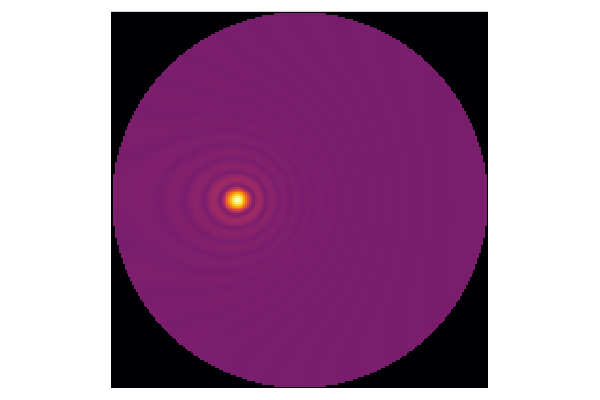
\includegraphics[width=\textwidth]{sample-reflectance}}
  \caption[Heatmap from the above sample code]{
    Heatmap of the reflectance found by the sample code above [\ref{chap:code}]}
\end{figure}

Talk about what the code does.

Talk about tests that validate that it should work.

Just include that section of the README here? As a usage example?

%%%%%%%%%%%%%%%%%%%%%%%%%%%%%%%%%%%%%%%%%%%%%%%%%%%%%%%%%%%%%%%%%%%%%%%%%%%%%%%%%%%%%%%%%%%%%%%%%%%%%%%%%%%%%%%%%%%%%%%%





% RESULTS %%%%%%%%%%%%%%%%%%%%%%%%%%%%%%%%%%%%%%%%%%%%%%%%%%%%%%%%%%%%%%%%%%%%%%%%%%%%%%%%%%%%%%%%%%%%%%%%%%%%%%%%%%%%%%

\chapter{Results}\label{chap:results}

Talk about condition numbers of impedance matrices.

%%%%%%%%%%%%%%%%%%%%%%%%%%%%%%%%%%%%%%%%%%%%%%%%%%%%%%%%%%%%%%%%%%%%%%%%%%%%%%%%%%%%%%%%%%%%%%%%%%%%%%%%%%%%%%%%%%%%%%%%





% CONCLUSION %%%%%%%%%%%%%%%%%%%%%%%%%%%%%%%%%%%%%%%%%%%%%%%%%%%%%%%%%%%%%%%%%%%%%%%%%%%%%%%%%%%%%%%%%%%%%%%%%%%%%%%%%%%

\chapter{Conclusion}\label{chap:conclusion}

Didn't work. Here are some ideas for making it work (need to come up with some, I'm not sure what to try).

%%%%%%%%%%%%%%%%%%%%%%%%%%%%%%%%%%%%%%%%%%%%%%%%%%%%%%%%%%%%%%%%%%%%%%%%%%%%%%%%%%%%%%%%%%%%%%%%%%%%%%%%%%%%%%%%%%%%%%%%





% APPENDICES %%%%%%%%%%%%%%%%%%%%%%%%%%%%%%%%%%%%%%%%%%%%%%%%%%%%%%%%%%%%%%%%%%%%%%%%%%%%%%%%%%%%%%%%%%%%%%%%%%%%%%%%%%%

\begin{appendices}

  \chapter{Circular Integration}\label{chap:circular_integration}
  
  What follows is Dr. Turley's work, which was foundational for this project and is referenced a bunch.
  
  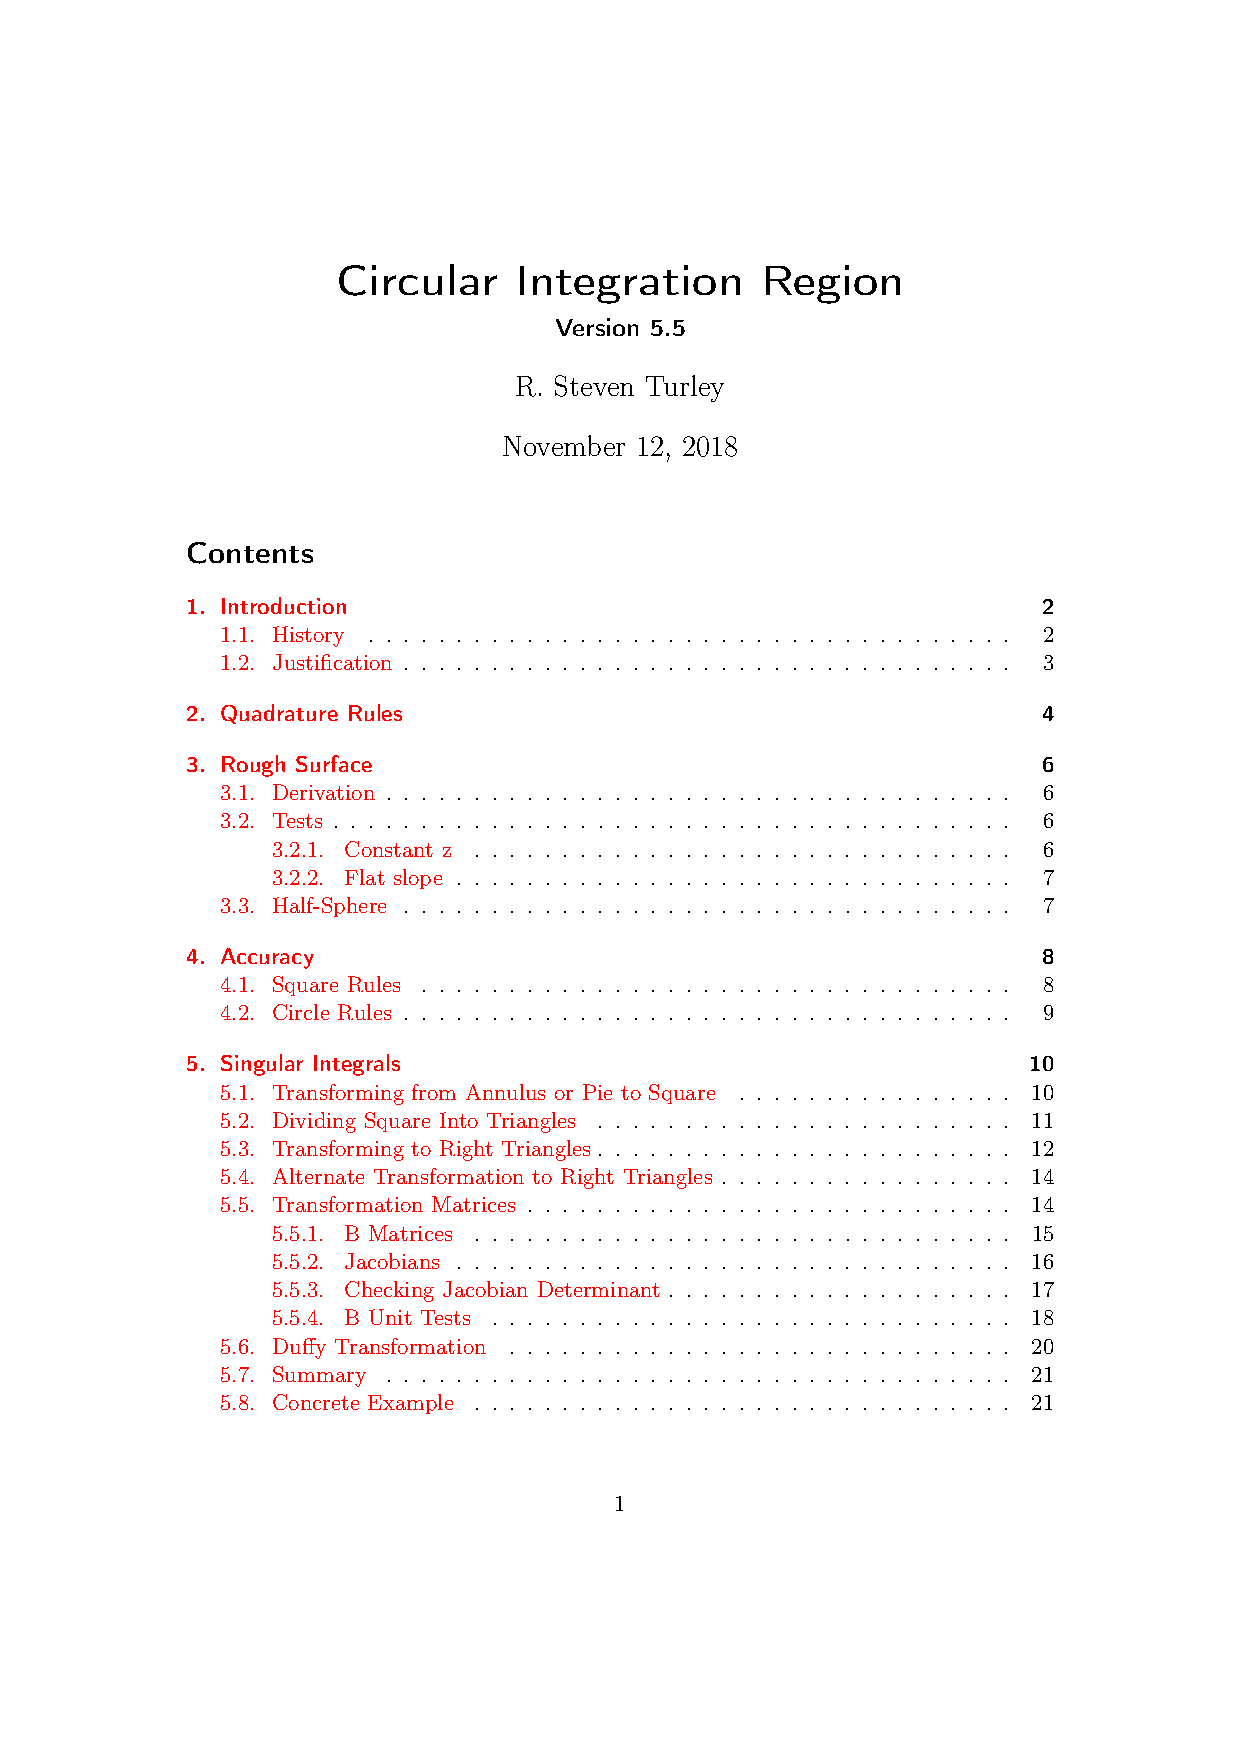
\includepdf[pages=-]{figures/circular-integration.pdf}
  
  
  
  \chapter{Generating Nice Heatmaps}\label{chap:heatmap_code}
  
  Given a \texttt{Reflectance} object \texttt{R}, a nice heatmap of said reflectance can be generated with:
  
  \begin{minted}{julia}
    heatmap((R.==0).*-max(R...)./2 + R, aspect_ratio=:equal,
                                        colorbar=false,
                                        xticks=false,
                                        yticks=false,
                                        axis=false,
                                        background=false)
  \end{minted}
  
  This was used to generate ONE? SEVERAL? figures in here.
  
  
  
  \chapter{Integral of Equation \ref{eq:integral1}}\label{chap:integral}
  
  Integration was done with Mathematica 13.1.0.
  
  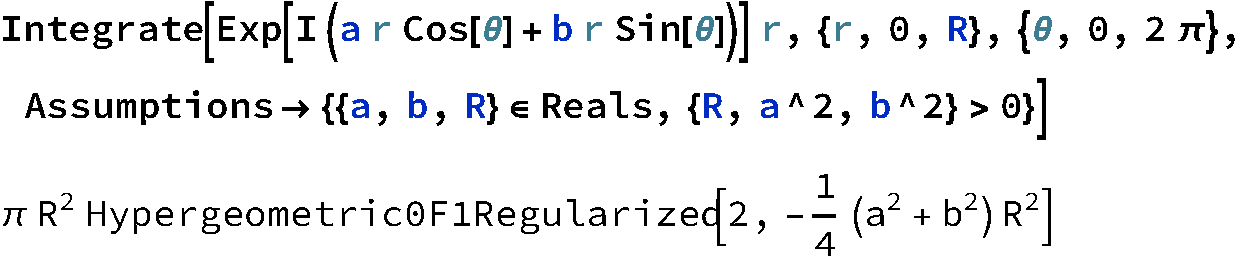
\includegraphics[width=\textwidth]{nasty-integral.pdf}
  
  
  
  \chapter{Simplification of Equation \ref{eq:expected_refl} Given Normal Light Incidence}\label{chap:airy_validation}
  
  Simplification was done with Mathematica 13.1.0.
  
  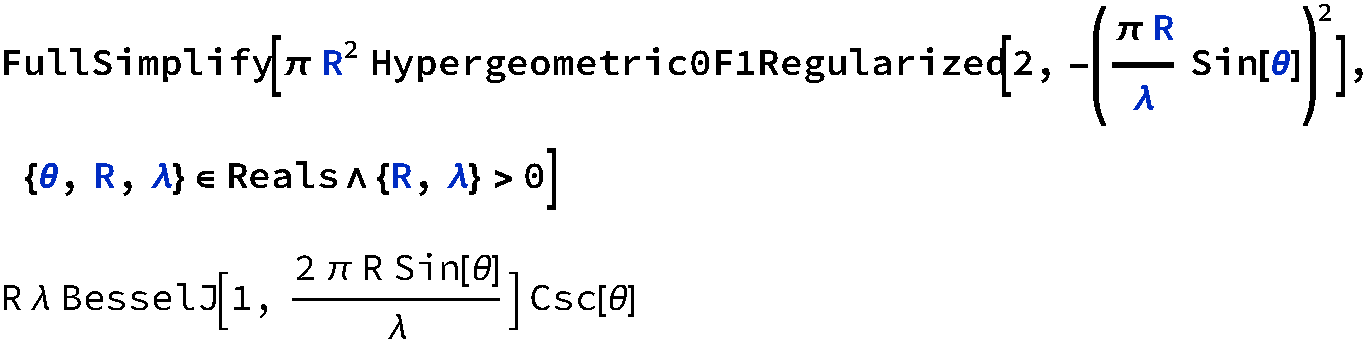
\includegraphics[width=\textwidth]{airy-simplification.pdf}
  
  
  
  \chapter{The Code}\label{chap:julia}
  
  \section{Structure}
  
  It's a fully functional Julia package. Here's the directory structure:
  
  \lstinputlisting{code-directory-structure.txt}
  
  \begin{tiny}
    \input{code.tex}
  \end{tiny}
  
\end{appendices}

%%%%%%%%%%%%%%%%%%%%%%%%%%%%%%%%%%%%%%%%%%%%%%%%%%%%%%%%%%%%%%%%%%%%%%%%%%%%%%%%%%%%%%%%%%%%%%%%%%%%%%%%%%%%%%%%%%%%%%%%





% Make the bibliography.
% Enter your references in the BibTex file "references.bib"
\bibliography{references}

% Make the index
\printindex

\end{document}
